\chapter{Požiadavky a návrh riešenia}

\label{kap:navrh_riesenia}

\section{Analýza požiadavkov}

Cieľom je vytvoriť webovú aplikáciu ktorá bude schopná vizualizovať výsledky meraní internetu v grafickej forme pomocou diagramov, 
grafov a máp. 

\subsection{Požiadavky na beh aplikácie}

Požiadavky na beh serverovej časti:
\begin{itemize}
    \item Systém musí byť schopný pracovať s PostgreSQL
    \item Systém nesmie zapisovať do databázy s meraniami
    \item Všetky časti systému musia byť schopné bežať na Linuxovom prostredí (CentOS alebo Ubuntu)
    \item Systém musí byť schopný priebežne predspracovávať namerané dáta po týždňoch, 
    aby boli vizualizácie zobrziteľné ihneď (bez dlhého čakania)
    \item Systém nesmie byť závislý od vonkajších servisov iných, ako databáza s meraniami 
    (lokalizačné servisy aj mapové servery musia bežať vrámci systému)
    \item Spracovanie dát pre jeden týždeň nesmie trvať viac ako jeden týždeň (nutné preto, aby spracovanie niekedy dobehlo)
\end{itemize}
Požiadavky na beh klientskej časti:
\begin{itemize}
    \item Aplikácia musí fungovať na všetkých moderných prehliadačoch
    \item Aplikácia musí vedieť vizualizácie zobrazovať bez pridlhého načitavania
\end{itemize}

Detaily implementácie boli ponechané na moje uváženie. Detaily rozhodovania sú popísané v kapitole \ref{kap:moznosti_implementacie}.

Serverový systém bude implementovaný na .NET 6.0. Systém bude pozostávať z niekoľkých aplikácií, z ktorých jedna bude pôsobiť ako 
server pre klientskú časť, jedna bude pôsobiť ako API pre získavanie spracovaných dát a zvyšné budú background workery, ktoré budú mať za úlohu
priebežne spracovávať namerané dáta. Predspracované dáta sa budú ukladať do PostgreSQL 15.0 databázy. Tieto workery budú spúšťané task schedulerom
jedenkrát týždenne. Systém bude bežať v niekoľkých kontaineroch v platforme Docker. Ako samostatný kontainer bude bežať databáza, API na prístup k 
dátam, nginx server pre klientskú aplikáciu, každý background worker a Open Street Maps tile server. Ako údaje na lokalizáciu ip adries bola 
použitá voľná databáza DB-IP lite \cite{ip_city_db}.

Klientská časť bude implementovaná pomocou systému Angular 15.0. API bude volané pomocou vstavanej knižnice httpClient. Na zobrazenie 
presnej geografickej mapy sveta budú použité Open Street Maps pomocou knižnice Leaflet a jej wrapperu pre Angular ngx-leaflet. Na zobrazenie 
mapy sveta po krajinách je použitý mierne upravený verejne voľný svg template \cite{svg_mapa}.

\section{Používateľské scenáre}
Keďže služby bežiace na pozadí nebudú mať žadneho používateľa a budú fungovať samy bez vstupu od používateľa, je potrebné navrhnúť len scenáre 
pre frontendovú aplikáciu.

\subsection{Používateľské scenáre pre frontendovú aplikáciu}
Aplikácia bude mať len jeden typ používateľa. Keďže celá webová čast je len na čítanie, nie je pootrebné obmedzovať práva pre niektorých používateľov. 
Z tohto dôvodu sme sa rozhodli vynechať autentifikáciu a aplikáciu sprístupniť bez mena a hesla.

\begin{itemize}
    \item Bežný používateľ - Po spustení aplikácie bude vidieť domovskú obrazovku. Tá bude pozostávať z navigačného menu, mapy sveta s vyznačenými skupinami 
    uzlov IP adries na základe ich geografickej polohy. Menu bude obsahovať dve položky, domovská obrazovka a mapa krajín. Na stránke bude prepínač týždňov, 
    ktorým sa bude ovládať voľba týždňa, pre ktorý chceme, aby sa dáta zobrazili. Tiež sa na stránke bude nachádzať výberový zoznam na výber medzi prezeraním 
    maximálnych, priemerných alebo minimálnych dôb odozvy. Po zmene stavu prepínačov sa zmeny v dátach prejavia okamžite pri všetkých troch selektoroch. 
    V mape sa tiež bude nachádzať legenda podľa ktorej sa bude dať určiť hodnota odozvy podľa farby kruhu znázorňujúceho uzol a počet IP adries reprezentovaných 
    kruhom podľa veľkosti priemeru kruhu.
    Po kliknutí na mapu krajín v menu sa zobrazí druhá stránka. Tá bude obshovať rovnaké menu ako domovská stránka. V hlavnej časti bude mapa krajín sveta. 
    Krajiny budú zafarbené podľa doby odozvy pre danú krajinu. Nad mapou sa bude nachádzať prepínač týždňov a rovnaké výberové zoznamy ako na domovskej stránke. 
    V mape sa tiež bude nachádzať legenda na priradenie doby odozvy k farbe.
\end{itemize}

\subsection{Návrh rozhrania na komunikáciu so serverovou časťou}
Rozhranie by malo fungovať podľa architektonického štýlu \uv{REST}. To určuje niekoľko pravidiel, medzi nimi napríklad oddelenosť backendu od frontendu, 
komunikáciu pomocou protokolu HTTP alebo nezávislosť dopytov jeden od druhého \cite{rest}. Rozhranie by malo obsahovať tieto metódy:
\begin{itemize}
    \item 
\end{itemize}

\subsection{Návrh lokálnej databázy}
Databázový pokytovateľ bude PostgreSQL vo verzií 15. Databáza bude bežať vo vyhradenom kontajneri. Databáza bude pozostávať z troch tabuliek. Prvá tabuľka 
sa bude volať \lstinline{ipadresses}. Bude slúžiť ako pomocná databáza pri napĺňaní zvyšných tabuliek. Bude obsahovať zoznam známych IP adries s informáciou 
o ich geografickej lokalite. Bude naplnená ko prvá, skôr ako zvyšné 2 tabuľky. Ďalšia tabuľka sa bude volať \lstinline{countrypinginfo} a bude obsahovať 
informácie o nameraných dobách odozvy zoskupených podľa krajín. Posledná tabuľka sa bude volať \lstinline{mapiprepresentation} a bude obsahovať informácie o nameraných dobách 
odozvy zoskupených podľa geografickej lokality. Tabuľky medzi sebou nebudú nijako prepojené, pretože by to neprinieslo žiadnu výhodu vzhľadom na charakter 
meraných dát. Entitno-relačný diagram je viditeľný na obrázku \ref{obr:entitn_diagram}.

Databáza bude obsahovať aj indexy. Indexy sú štruktúra, ktorá umnožňuje zrýchliť vyhľadávanie v databáze na úkor spomalenia zápisu \cite{db_index}. 
Čas nás v násom systéme zaujíma hlavne z hľadiska používania webovej aplikácie. Tá z databázy výlučne číta. Zápis budeme naopak robiť len raz do týždňa 
a na čase pri ňom príliš nezáleží (jediné obmedzenie je, že spracovanie týždňa musí trvať menej ako týždeň, čo je veľmi štedrý čas). Vzhľadom na to je 
takáto optimalizácia v našom systéme veľmi vítaná. Keďže systém môže bežať dlhý čas, spracované údaje sa môžu stať priveľké a vyhľadávanie v nich bez 
indexácie by bolo veľmi pomalé. Zároveň jednoznačné indexy vedia zaručiť väčšiu konzistentnosť dát, keďže vedia zaručiť, že kombinácie niektorých údajov 
sa môžu v tabuľke vyskytnúť maximálne raz \cite{index_strategy}.

Okrem primárneho kľúča v každej tabuľke ich bude 5. Pôjde o index zaručujúci jedinečnosť IP adresy v tabuľke 
\lstinline{ipadresses}, index zaručujúci jedinečnosť kombinácie zemepisnej šírky, dĺžky a týždňa v tabuľke \lstinline{mapiprepresentation}, index na 
optimalizáciu vyhľadávania podľa týždňa v tabuľke \lstinline{mapiprepresentation}, index zaručujúci jedinečnosť kombinácie krajiny a týždňa v tabuľke 
\lstinline{countrypinginfo} a index na optimalizáciu rýchlosti vyhľadávania podľa týždňa v tabuľke \lstinline{countrypinginfo}.

\begin{figure}
    \centerline{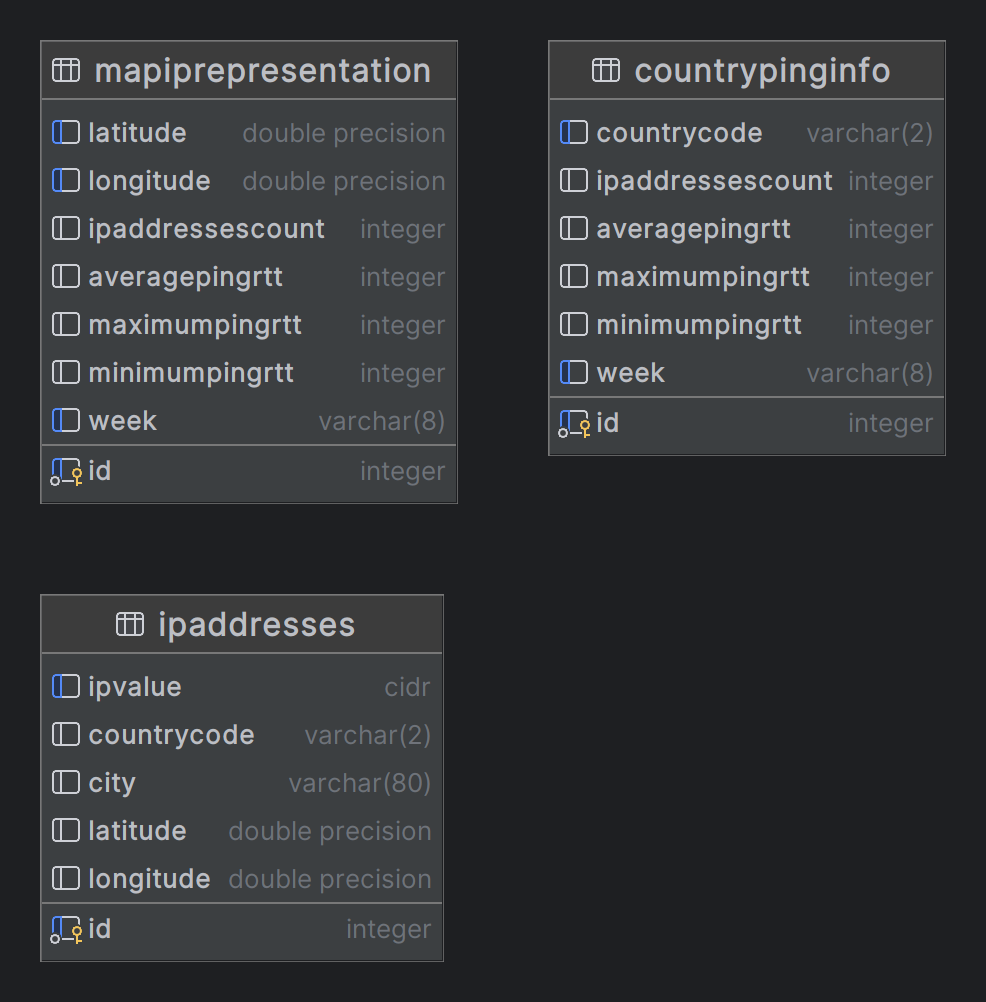
\includegraphics[width=0.8\textwidth]{images/ipinfoviewerprocesseddb}}
    %popis obrazku
    \caption[Entitno-relačný digram k lokálnej databáze]{Na obrázku je vidno, že tabuľky nie sú nijako previazané}.
    %id obrazku, pomocou ktoreho sa budeme na obrazok odvolavat
    \label{obr:entitn_diagram}
\end{figure}